\title{Trending topics using the Twitter-API}
\author{
        Marco Pock-Steen Fraile \\
        Christian Palmh\o j Nielsen \\
        IT University of Copenhagen\\
}
\date{\today}

\documentclass[12pt]{article}

\usepackage{graphicx}
\usepackage{algpseudocode}
\usepackage{algorithm}

\begin{document}
\maketitle

\begin{abstract}
We have designed an algorithm for identifying trending topics in twitter..
\end{abstract}

\section{Introduction}
We wish to make use of the Twitter streaming API to analyze messages and find trending topics, as well as

We wish to make use of the Twitter streaming API to implement our own version of trending topics using the Misra-Gries algorithm, and for the trending topics we would track how many unique tweets have been made per topic, using one of the algorithms for counting distinct elements. We could also count number of tweets for trending topics to compare actual tweets with unique tweets, but this is not algorithmically a challenge.
\newline\newline
Challenges would include finding a suitable k for the Misra-Gries that is a good trade-off between memory space and making sure we take into account the tweets inbetween the actual trending topics that might "flood" them out of the array.
\newline\newline
For the counting algorithm we similarly need to find a good hashing algorithm for tweets, and based on this find a good number for kth-minimum distances that gives us a realistic count for unique tweets.

\paragraph{Outline}
The remainder of this article is organized as follows.
Section~\ref{related work} gives account of previous work.
Our new and exciting results are described in Section~\ref{results}.
Finally, Section~\ref{conclusions} gives the conclusions.


\section{Twitter}
Twitter is a real-time information network that connects you to the latest stories, ideas, opinions and news about what you find interesting. All information on Twitter is distributed through ``tweets'', small 140-character messages where a person can shortly state an opinion, an event or random thoughts. Because of the format, twitter encourages frequent updates from users and as of October 26th, 2012 around 500 million tweets are written per day (24 hours)\cite{Cnet1}. With 140 million users, this means each user, on average, posts 3.5 tweets per day. A typical tweet can be seen below.

\newline
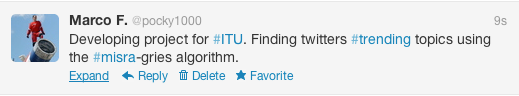
\includegraphics[width=125mm]{tweet.png}
\newline

Each user on twitter chooses other users to follow and see an aggregated list of all their tweets. Tweets can be replied to by in this form: \quote{@pocky1000 You are totally right. #ITU is super cool.}

\subsection{Hashtags and topics}
For the purpose of categorizing tweets, users put hashtags within their tweets. Examples include, as seen above, \#ITU, \#trending and \#Misra. For the purpose of this paper, we will consider these hashtags as topics, and will only consider tweets that contain at least one hashtag. If a tweet contains several hashtags, we will consider each one seperately, but will use the entire tweet when considering distinct tweets.

<<<<<<< HEAD
Users of twitter can see the tweets of people they follow, and have the options to either reply to a tweet, or retweet it. On retweet the user basically shares the same message to their own followers, giving credit to the creator of the message.
The topic of a tweet is identified by the presence of a hashtag \# in front of a word. In the example above the topics are \#ITU,\#trending and \#Misra.
Tweets can be tagged by writing a hashtag ``\#'' followed by a topic or keyword. Twitter users this as a way to categorize messages.
A trending topic is defined by a topic that has a high frequency, in other words many people are ``tweeting'' about the same topic at some point in time. A trending topic can either be many unique tweets about the same topic, e.g. if people are tweeting to promote some beneficial cause, or it can be the same message retweeted by many users.
Twitter currently have over 500 million users, so the amount of tweets produced at any moment is equally big, some specifics. We use the public Twitter API to create a stream of which corresponds to a sample of all tweets. 
=======
A trending topic is defined by a topic that has a high frequency, in other words many people are ``tweeting'' about the same topic over a period of time. This topic can be used by many individuals to give their input, and as such will have many unique tweets, or it can be a specific message that has been re-tweeted a lot of times.
>>>>>>> 546d0f257e0a50c4c637c7af191ab84f874188e8

\section{Streaming algorithms}\label{related work}
Twitter and other social networks are structured to accomodate personal communication across large networks of friends, and a such produce enormous amounts of data. The open availability of this data through developer APIs makes it's an interesting source for useful real-time information extraction using streaming algorithms. \cite{genderprediction} 
This section introduces the concepts of algorithms that can compute some function of a massively long input stream $\sigma$ such as all public available tweets. In our model this is formalized as a sequence $\sigma = \langle a_{1}, a_{2},...,a_{m}\rangle $, where the elements of the sequence (called $tweets$) are drawn from the universe $[n] =: \{1, 2,..., n\}$. Note the two size parameters: the stream length, $m$, and the universe size, $n$.
Our goal will be to process the input stream using a small amount of space $s$, i.e., to use s bits of random-access working memory. Since $m$ and $n$ are to be thought of ``huge'' we want to make $s$ much smaller than these. Ideally we want to achieve $s$ = O(log $m$ + log $n$), because this is the amount of space needed to store a constant number of elements from the stream and a constant number of counters that can count up to the length of the stream. \cite{Amit}

\subsection{Finding frequent items}
We want to find the the frequency of certain terms in each $tweet$ in our input stream $\sigma = \langle a_{1}, a_{2},...,a_{m}\rangle$, and define a frequency vector $f = (f_{1},...,f_{n})$, where $f_{1} + ... + f_{n} = m$. 

The Misra-Gries Algorithm solves the problem of estimating the frequencies $f_{j}$ \cite{Amit}

A similar scoring method is suggested where a topic is given a score based on the frequency over a period of time. That means that if a topic generally has a high frequency over a long period of time, it will not necessarily be considered trending if a topic with a lower frequency gained it over a shorter period of time. The standard score is defined as $z = \frac{x - \mu}{\sigma}$, where $x$ is the raw score, $\mu$ is the mean of the population and $\sigma$ is the standard of the population.

\subsection{Finding distinct values}
K-minimum values (KMV) is is a probalistic distinct value counting algorithm, that is intuitive and easy to implement \cite{kmv}. Suppose we have a good hash function that return evenly distributed values in the hash space $[0-1]$, then you could estimate the number of distinct values you have seen by knowing the average spacing between values in the hash space. The main challenge is to find a good hash function, and to select the number of minimum $k$ values on which to approximate the average spacing. If the hash values were indeed evenly distributed, we could keep just keep track of the minimum value, a get a good estimate of distinct values. However taking only one value opens up to a lot of variance and would rely heavily upon the``goodness'' of the hash function. In order to improve this Bar-Yossef\cite{Bar-Yossef} suggests keeping the k-smallest values, to give a more realistic estimate.
   
Other examples of the usages of data stream algorithms are described in this chapter.
\subsection{Misra-Gries Algorithm}
The algorithm first initializes a dictionary with $k$ number of values. The keys in the dictionary are elements seen in the stream, and the value are counters associated with the elements. Then there is a process function that is executed each time we see a new element. If a new element is already in the dictionary, it's value will be increased by 1, otherwise if the number of elements in $A$ is less than $k$, the element will be inserted an its value set to 1. If the length of $A$ is equal to $k$, all values are decreased by 1, and removed if the value is equal to 0. \cite{Amit}.Finally we return the key value pairs with the highest frequencies.
\begin{algorithm}
\caption{Misra-Gries Algorithm}
We use Misra-Gries to find frequent $topics$ in our data stream of tweets using a one-pass algorithm.
\begin{algorithmic}
\State $A\gets Initialize Array$

\Function{Process}{$j$}
\If {$j \in keys(A)$}
	\State $A[j] \leftarrow A[j] + 1$
\ElsIf {$|keys(A)| < k-1 $}
	\State $A[j] \leftarrow 1$
\Else
	\For{$l \in keys(A)$}
		\State {$A[l] \leftarrow A[l] - 1$}
		\If {$A[l] = 0$} remove $l$ from A
		\EndIf
	\EndFor
\EndIf
\EndFunction
\end{algorithmic}
\end{algorithm}

\subsection{Analysis of algorithm}

\subsection{Rising trends}
Varying $k$ to change the amount of time the trending topics cover.

\subsection{Data structure}
When a new tweet is registered the algorithm has to determine if the contained topic has already been seen. We need a data structure that provides fast lookup, such as a dictionary with key-value pair as topic-frequency. We also need to find a data structure that allows for decrementing all values by 1 if the topic is not already created. Lastly we will have to find a way to randomly remove a topic if the data structure exceeds k at the creation of a new topic.

\subsection{Data Set}

\section{Results}\label{results}
In this section we describe the results.

\section{Conclusions}\label{conclusions}
We worked hard, and achieved very little.

\bibliographystyle{abbrv}
\bibliography{simple}

\end{document}
This is never printed